\section{Zielsetzung}
  \label{sec:Zielsetzung}
  Im diesem Versuch wird zuerst ein Sagnac-Interferometer nach den in der Anleitung beschriebenen Schritten aufgebaut/justiert.

  Dann wird der Kontrast $K(\phi)$ des Interferometers in Abh"angigkeit des Winkels $\phi$ des ersten (und einzigen) Polarisationsfilters vor dem PBSC (f"ur eine ganze Periode von K von $\SI{0}{\degree}$ bis $\SI{90}{\degree}$) gemessen, indem f"ur 10 Winkel im Messbereich je die minimale/maximale Spannung der Photodiode auf die der Output-Beam trifft notiert wird.

  Danach wird der Brechungsindex von Glas und Luft (bei Atmospherendruck) bestimmt, bei fester Einstellung des Polarisationsfilterwinkels, f"ur maximalen Kontrast $K$.
  Daf"ur wird die Anzahl der Interferenzaxima/-minima, mit einer Glasplatte in jedem der beiden Strahlen des Interferometers, in Abh"angigkeit des Winkels $\theta$ der Platten bez"uglich der Strahlen bestimmt.

  Und es wird die Anzahl der Interferenzmaxima/-minima in Abh"angigkeit des Luftdruckes in einem Rohr gemessen, welches von einem der Strahlen durchlaufen wird.




\section{Theorie}
  \label{sec:Theorie}
  \subsection{Licht als elektromagnetische Welle}
    Der vorligende Versuch basiert auf Interferometrie, das hei"st der Aunsutzung der Interferenzeffekte von elektromagnetischen Wellen zum Bestimmen von Messgr"o"sen.
    Interferenz ist die "Uberlagerung/Supersposition von Wellen und kann bei Licht daher nur mit der Wellennatur des Lichtes beschrieben werden (also nicht im Rahmen der geometrischen Optik).

    F"ur die zeitlich gemittelte Intensit"at $I$ zweier interferienrender linear polarisierter elektromagnetischer Wellen ergibt sich die Formel
    \begin{equation}
      I \propto \left<\left|\vec{E_1}+\vec{E_2}\right|^2\right>
      =E_{01}^2 + E_{02}^2 + 2E_{01}E_{02}\cos{(\delta)}\cos{(\Phi)} \; ,
      \label{intensitaet}
    \end{equation}
    mit den Amplituden $E_{01}/E_{02}$ des E-Feldes von Welle 1 und 2, welche dem Betrag des E-feld-Vektors entspricht.
    $\Phi$ ist die (ortsabh"angige) Phasenverschebung der (E-Feld-)Wellen und $\delta$ ist der Winkel zwischen den Polarisationsachsen der beiden Wellen.
    F"ur senkrecht zueinander polarisierte Wellen ($\delta=\pi/2=\SI{90}{\degree}$) ist die Intensit"at $I$
    \begin{equation}
      I \propto E_{01}^2 + E_{02}^2 \; ,
    \end{equation}
    also unabh"angig von der Phasenverschiebung (und somit unabh"angig vom Ort), was bedeutet, dass es hier keine Interferenzeffekte gibt.

    \subsubsection{Polarisation elektromagnetischer Wellen}
      Polarisation bezeichnet im Allgemeinen die Ausrichtung des E-Feld-Vektors $\vec{E}$ einer elektromagnetischen Welle in der Ebene senkrecht zur Ausbreitungsrichtung, also parallel  zum Wellenvektor $\vec{k}$.
      Da der $\vec{E}$ immer senkrecht zu $\vec{k}$ steht (und auch senkrecht zu $\vec{B}$), kann man den E-Feld-Vektor, in einem Koordinatensystem mit z-Achse parallel zur Ausbreitungsrichtung, allgemein schreiben als:
      \begin{equation}
        \vec{E}= \left( \begin{array}{c}E_x\sin{(\omega t)}\\E_y\sin{(\omega t + \alpha)}\\0\end{array} \right)
      \end{equation}
      Linear polarisiertes Licht ergibt sich f"ur $\alpha=0$, dann "andert sich nur die L"ange des Vektors mit der Zeit, die Richtung bleibt konstant.

    \subsubsection{Brechungsindex $n$ von Materie}
      Der Brechungsindex von Materie ist das Verh"altnis zwischen Vakuumslichtgeschwindigkeit $c=const$ und Lichtgeschwindigkeit $v$ in dieser Materie:
      \begin{equation}
        n=\frac{c}{v}
        \label{brechungsindex}
      \end{equation}




  \subsection{Interferometer}
    \subsubsection{Kontrast eines Interferometers}
      Der Kontrast $K$ eines Interferometers ist definiert als
      \begin{equation}
        K = \frac{I_{max}-I_{min}}{I_{max}+I_{min}}
        \label{kontrast}
      \end{equation}
      Hierbei sind $I_{min/max}$ die minimale/maximale Intensit"at des linear polarisierten Output-Strahls des Interferometers.
      Es ist zu erkennen, dass der ideale Kontrast 1 betr"agt, da im Idealfall $I_{min}=0$ ist.
      Je n"aher $K$ in der Praxis an 1 ist, desto besser.

      Durchquert der Laserstrahl im Interferometer einen Polarisationsfilter, werden $I_{min/max}$ von dem Winkel $\phi$ des Filters bzw. seiner Polarisationsachse zu der E-Feld-Achse des Strahls abh"angen, da ein Polarisationsfilter nur Licht hindurchl"asst. welches senkrecht zur seiner Polarisationsachse polarisiert ist.
      Um die Abh"angigkeiten zu erreichen wird von der allgemeinen Intensit"at $I$ zweier interferierender Strahlen/Wellen ausgegangen (Formel (\ref{intensitaet})).
      Im Versuch enstehen die zwei Wellen mit E-Feld Amplituden $E_{01/02}$ durch das Aufteilen eines Strahls mit urspr"unglicher E-Feld Amplitude $E$ am PBSC (in zwei zueinander im Winkel $\delta = \pi /2$ polarisierte Strahlen), nachdem dieser einen Polarisationsfilter im Winkel $\phi$ durchlaufen hat, somit folgt
      \begin{align}
        E_{01} &= E\cos(\phi)\\
        E_{02} &= E\cos{(\phi - \frac{\pi}{2})} = E\sin(\phi) \; .
      \end{align}
      Dadurch wird $I$ aus (\ref{intensitaet}) zu:
      \begin{equation}
        I = E^2(1+\cos(\phi)\sin(\phi)\cos(\Phi))
      \end{equation}
      Die maximale Intensit"at wird erreicht, wenn die Phasenverschiebung der beiden Strahlen/Wellen $\Phi$ null ist, die minimale bei $\pi$, das hei"st wenn der Cosinus ist $\pm 1$.
      Durch Einsetzen von $I_{max/min}$ in (\ref{kontrast}) kann der Kontrast $K$ vereinfacht werden zu
      \begin{equation}
        K = E^2\sin{(2\phi)} \propto \sin{(2\phi)} \; .
        \label{kontrast2}
      \end{equation}

    \subsubsection{Bestimmung von Brechungsindizes mit einem Interferometer}
      Durchl"auft einer der Laserstrahlen (des durch den PBSC aufgeteilten Ursprungsstrahls) auf einer Strecke ein anderes Medium mit anderem Brechungsindex, ergibt sich nach (\ref{brechungsindex}) eine andere Lichtgeschwindigkeit des Strahls auf dieser Strecke, dadurch "andert sich der Betrag des Wellenvektors zu
      \begin{equation}
        k_{neu}=k \cdot n \; .
      \end{equation}
      Damit "andert sich die Phase der Strahlen zueinander um $\Delta \phi$ und somit auch die Anzahl $M$ der Interferenzmaxima/-minima, welche entstehen, wenn die Strahlen (ebene Wellen) wieder aufeinander treffen (und nicht senkrecht zueinander polarisiert sind).\\
      \\Durchl"auft einer der Strahlen im Interferometer auf der L"ange $L$ ein Gas mit Brechungsindex $n$, ergibt sich der Zusammenhang
      \begin{equation}
        M=2\frac{\Delta \phi}{2 \pi}=\frac{n-1}{\lambda_{vak}}(2L)
        \label{gas}
      \end{equation}
      mit der Vakuumswellenl"ange des Lichtes $\lambda_{vak}$.\\
      \\Durchl"auft einer der Strahlen im Interferometer eine Glasplatte mit Dicke $T$, welche im Winkel $\theta$ (im Gradma"s) im Strahl ist (siehe Abb. \ref{fig:glasplatte}) ergibt sich n"aherungsweise
      \begin{equation}
        M \approx 2\frac{T}{\lambda_{vak}} \frac{n-1}{n}\left(\theta \frac{2\pi}{360}\right)^2 \;
        \iff n = \frac{1}{1-\frac{M\lambda_{vac}}{2T\left(\theta\frac{2\pi}{360}\right)^2}}
        \label{glas}
      \end{equation}
      %BEI ZWEI GLASPLATTEN DAS DOPPELTE, ABER IN ALTPROT IST DAS HIER SCHON DAS DOPPELTe?????????
      \begin{figure}[H]
        \centering
        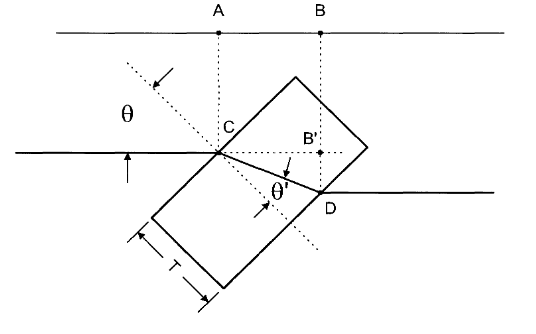
\includegraphics[height=5cm]{bilder/glasplatte.png}
        \caption{Strahlengang an einer Glasplatte der Dicke $T$, im Winkel $\theta$ zur Senkrechten des Strahls \cite{Anleitung}.}
        \label{fig:glasplatte}
      \end{figure}
